\documentclass[10pt]{article}
\usepackage[letterpaper,margin=0.8in]{geometry}
\usepackage[T1]{fontenc}
\usepackage{lmodern,amsmath,booktabs,graphicx,caption,float,microtype}
\usepackage[colorlinks=true,urlcolor=blue,linkcolor=black]{hyperref}
\setlength{\parindent}{0pt}
\setlength{\parskip}{4pt}
\captionsetup{font=small,labelfont=bf}
% Generated by code/run_question1.py
\newcommand{\RawRows}{1,114,194}
\newcommand{\RawBanks}{17,804}
\newcommand{\PanelRows}{1,105,619}
\newcommand{\PanelBanks}{17,620}
\newcommand{\OtherCharters}{8,575}
\newcommand{\Gaps}{133}
\newcommand{\BanksFirst}{13,342}
\newcommand{\BanksLast}{4,114}
\newcommand{\AssetsFirst}{1.92}
\newcommand{\AssetsLast}{13.34}
\newcommand{\CoreEligible}{10,399}
\newcommand{\CoreExcluded}{7,221}
\newcommand{\RoaEligible}{10,439}
\newcommand{\LinkedBanks}{5,121}
\newcommand{\LinkedCompanies}{1,061}
\newcommand{\MarketBanks}{1,706}
\newcommand{\MarketCompanies}{691}
\newcommand{\MarketObservations}{64,230}
\newcommand{\IncompleteGroups}{608}
\newcommand{\StockDuplicates}{556}
\newcommand{\MarketLastIndex}{139.7}
\newcommand{\IncMean}{0.369}
\newcommand{\IncMedian}{0.354}
\newcommand{\ExpMean}{0.356}
\newcommand{\ExpMedian}{0.352}
\newcommand{\RoaMean}{0.025}
\newcommand{\RoaMedian}{0.007}
\newcommand{\IncAllSlope}{0.696}
\newcommand{\IncAllIntercept}{0.122}
\newcommand{\IncAllRsq}{0.206}
\newcommand{\IncSmallSlope}{0.612}
\newcommand{\IncSmallIntercept}{0.140}
\newcommand{\IncSmallRsq}{0.142}
\newcommand{\IncLargeSlope}{0.734}
\newcommand{\IncLargeIntercept}{0.118}
\newcommand{\IncLargeRsq}{0.248}
\newcommand{\RoaAllSlope}{0.142}
\newcommand{\RoaAllIntercept}{-0.025}
\newcommand{\RoaAllRsq}{0.002}
\newcommand{\RoaSmallSlope}{-0.051}
\newcommand{\RoaSmallIntercept}{0.024}
\newcommand{\RoaSmallRsq}{0.000}
\newcommand{\RoaLargeSlope}{0.261}
\newcommand{\RoaLargeIntercept}{-0.054}
\newcommand{\RoaLargeRsq}{0.009}
\newcommand{\SizeCutoff}{83.4}
\newcommand{\RawIncSlope}{0.796}
\newcommand{\RawIncT}{5.44}
\newcommand{\RawRoaSlope}{-0.380}
\newcommand{\RawRoaT}{-0.46}
\newcommand{\StockSize}{-0.628}
\newcommand{\StockRoa}{0.034}
\newcommand{\StockCapital}{-0.043}

\begin{document}
\begin{center}\Large Question 1: Bank Interest-Rate Sensitivity\end{center}
\vspace{-0.5em}

\section*{Part 1. Data audit and descriptive evidence}
The accounting file contains \RawRows{} observations for \RawBanks{} banks, with unique bank--quarter keys and no missing identifiers. I retain commercial-bank records (\texttt{charter\_type = 200}), excluding \OtherCharters{} other or unclassified records.\footnote{Charter coding: \href{https://www.ffiec.gov/npw/StaticData/DataDownload/NPW\%20Data\%20Dictionary.pdf}{Federal Reserve NIC data dictionary}, charter-type definition.}
The resulting unbalanced panel has \PanelRows{} observations for \PanelBanks{} banks over 1984Q1--2017Q4.

Table~\ref{tab:descriptive} shows a strongly skewed size distribution. Figure~\ref{fig:industry} shows the number of reporting commercial banks falling from \BanksFirst{} to \BanksLast{}, while nominal assets rise from \$\AssetsFirst{} trillion to \$\AssetsLast{} trillion. This pattern is consistent with consolidation, although entry, exit, charter changes and inflation also affect the series; it does not identify mergers separately.

I convert year-to-date (YTD) interest income, interest expense and net income into quarterly flows before imposing the charter restriction.\footnote{YTD reporting: \href{https://www.fdic.gov/system/files/2024-08/2008-06-ri.pdf}{FFIEC Schedule RI instructions}, general instructions.} Q1 equals the reported amount; later quarters equal current minus immediately preceding YTD amounts within the same year. A missing predecessor leaves the quarterly flow unavailable. Positive, finite average assets are required for rates. Negative quarterly interest flows are treated as unavailable because reporting resets or revisions can make them misleading; zero interest and negative net income remain valid.

To limit the influence of extreme ratios, I cap income and expense rates at each quarter's 99.5th percentile and ROA at its 0.5th and 99.5th percentiles, before differencing. This preserves zero interest and ordinary losses but can attenuate genuine tail responses. Part 3 reports a check without these caps. No missing values are imputed. Figure~\ref{fig:missing} measures missingness among observed records; it excludes absent quarters. There are \Gaps{} internal gaps between retained bank reports. Bank exits, changing reporting populations and the later minimum-history requirement limit representativeness.

\begin{table}[H]
\centering
\caption{Main descriptive statistics}\label{tab:descriptive}
\resizebox{\textwidth}{!}{\begin{tabular}{lrrrrrrr}
\toprule
 & N & Mean & SD & P25 & Median & P75 & Missing (\%) \\
Variable &  &  &  &  &  &  &  \\
\midrule
Average assets (USD bn) & 1,105,584 & 0.751 & 20.374 & 0.031 & 0.066 & 0.155 & 0.003 \\
Total assets (USD bn) & 1,105,588 & 0.759 & 20.547 & 0.031 & 0.066 & 0.157 & 0.003 \\
Equity/assets (\%) & 1,105,588 & 10.340 & 6.518 & 7.690 & 9.164 & 11.276 & 0.003 \\
Quarterly interest income (USD mn) & 1,100,247 & 9.710 & 188.524 & 0.581 & 1.181 & 2.569 & 0.486 \\
Quarterly interest expense (USD mn) & 1,100,247 & 3.537 & 69.719 & 0.215 & 0.462 & 1.023 & 0.486 \\
Quarterly net income (USD mn) & 1,100,248 & 1.794 & 56.560 & 0.050 & 0.152 & 0.405 & 0.486 \\
Income rate (\%) & 1,098,645 & 7.420 & 2.226 & 5.805 & 7.532 & 9.034 & 0.631 \\
Expense rate (\%) & 1,098,622 & 3.404 & 1.911 & 1.924 & 3.343 & 4.936 & 0.633 \\
ROA (\%) & 1,100,242 & 0.818 & 1.569 & 0.584 & 1.038 & 1.438 & 0.486 \\
Change in income rate (pp) & 1,079,586 & -0.054 & 0.642 & -0.251 & -0.036 & 0.153 & 2.355 \\
Change in expense rate (pp) & 1,079,537 & -0.048 & 0.323 & -0.163 & -0.033 & 0.068 & 2.359 \\
Change in ROA (pp) & 1,082,555 & 0.000 & 1.611 & -0.277 & 0.009 & 0.280 & 2.086 \\
Fed funds (\%) & 136 & 3.869 & 3.022 & 0.932 & 4.200 & 5.893 & 0.000 \\
Change in Fed funds (pp) & 136 & -0.060 & 0.555 & -0.193 & -0.005 & 0.150 & 0.000 \\
Monthly stock return (pp) & 64,230 & 0.953 & 10.782 & -3.489 & 0.625 & 5.027 & 0.000 \\
Log company assets (USD thousand) & 64,230 & 14.359 & 1.686 & 13.295 & 14.088 & 15.182 & 0.000 \\
\bottomrule
\end{tabular}
}
\begin{minipage}{\textwidth}\footnotesize
Bank variables use observed commercial-bank quarters. Dollar flows retain original deaccumulated amounts; rate levels and changes use the cleaning described above. Policy variables have one observation per quarter. Stock returns and log company assets use the final company--month sample. USD amounts are nominal; pp denotes percentage points. Missing percentages use the relevant observation unit, rather than a balanced panel.
\end{minipage}
\end{table}

\begin{figure}[H]
\centering
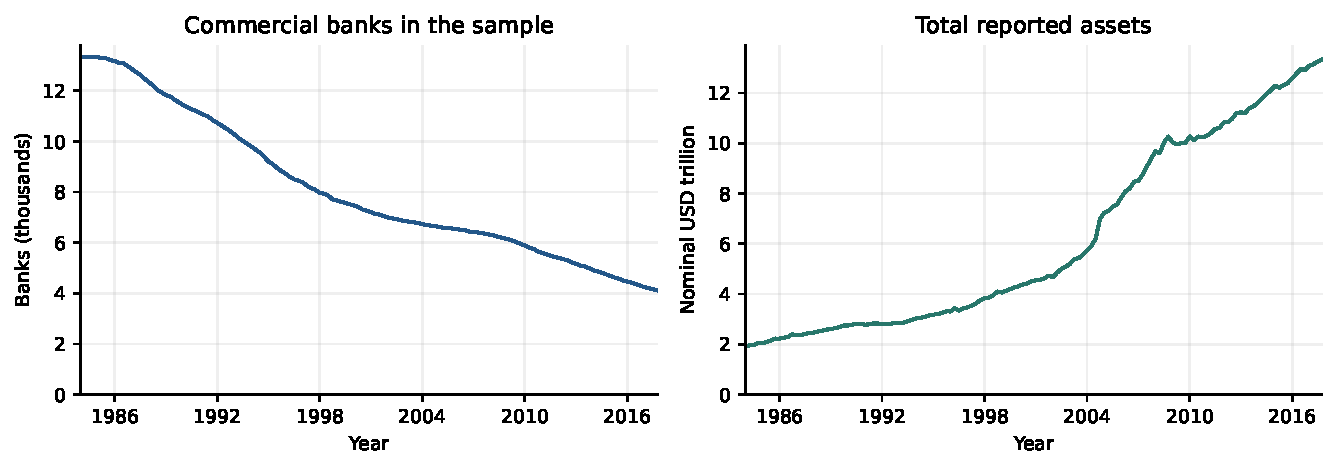
\includegraphics[width=0.92\textwidth]{figures/industry.pdf}
\caption{Commercial-bank counts and summed positive reported total assets.}\label{fig:industry}
\end{figure}
\begin{figure}[H]
\centering
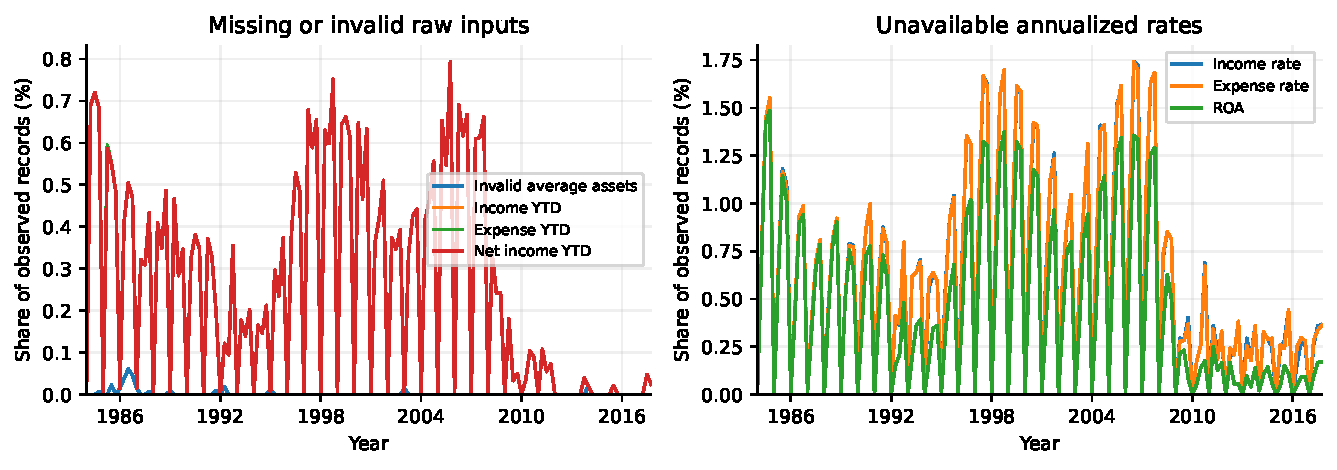
\includegraphics[width=0.92\textwidth]{figures/missingness.pdf}
\caption{Missing or invalid raw inputs and unavailable constructed rates, by quarter. Rates also require quarterly flows and valid assets.}\label{fig:missing}
\end{figure}

\section*{Part 2. Bank-level income and expense betas}
For quarterly flow $Q^y_{it}$ and quarterly average assets $A_{it}$, I construct
\[
 y_{it}=400\frac{Q^y_{it}}{A_{it}},\qquad
 \Delta y_{it}=y_{it}-y_{i,t-1},\qquad
 \Delta f_t=f_t-f_{t-1}.
\]
Rates and changes are in percentage points. A bank difference is valid only across consecutive calendar quarters, including Q4 to Q1. The policy rate $f_t$ is the supplied monthly rate for March, June, September or December, not a quarterly average. A complete quarterly policy calendar is merged many-to-one into the bank panel; 1983 observations construct the initial changes and lags.

For each bank and each outcome, I estimate
\[
 \Delta y_{it}=a_i^y+\sum_{\tau=0}^{3}b^y_{i\tau}\Delta f_{t-\tau}+u^y_{it},
 \qquad \widehat\beta_i^y=\sum_{\tau=0}^{3}\widehat b^y_{i\tau}.
\]
Income and expense regressions use the same finite observations within each bank. I require at least 40 usable quarters and full regressor rank: ten years of observations improves precision relative to fitting five parameters to very short histories, while retaining an unbalanced sample. This yields \CoreEligible{} banks; \CoreExcluded{} have insufficient observations. Each bank has its own intercept and slopes. Calendar-quarter fixed effects would absorb the common policy changes, preventing identification. The intercept is excluded from the beta sum.

\begin{table}[H]
\centering
\caption{Distribution of estimated cumulative responses}\label{tab:betas}
\begin{tabular}{lrrrrrrrr}
\toprule
 & Banks & Mean & SD & P25 & Median & P75 & \shortstack{Median\\HAC SE} & \shortstack{Significant\\(\%)} \\
\midrule
Income beta & 10,399 & 0.369 & 0.159 & 0.276 & 0.354 & 0.447 & 0.082 & 86.0 \\
Expense beta & 10,399 & 0.356 & 0.104 & 0.298 & 0.352 & 0.410 & 0.052 & 95.7 \\
ROA beta & 10,439 & 0.025 & 0.293 & -0.086 & 0.007 & 0.110 & 0.167 & 2.8 \\
\bottomrule
\end{tabular}

\begin{minipage}{0.94\textwidth}\footnotesize
Equal weight per eligible bank; no filtering by statistical significance. ROA uses its own available quarters, with the same 40-quarter threshold. All betas are outcome percentage points per policy percentage point.
\end{minipage}
\end{table}

Mean income and expense betas are \IncMean{} and \ExpMean{}; their medians are \IncMedian{} and \ExpMedian{}. A one-percentage-point permanent rise in the policy-rate level is therefore associated with \IncMean{} pp higher income rates and \ExpMean{} pp higher expense rates after four quarters for the average eligible bank. These are asset-scaled rates, so the expense beta is not a deposit-rate beta. Similar average responses suggest substantial offsetting repricing of income and costs. The estimates are descriptive: policy responds to economic conditions, banks face shared shocks, and bank-specific sample windows differ. The required one-row-per-bank income/expense estimates are in \texttt{bank\_betas.csv}.

\section*{Part 3. Cross-sectional analysis and market data}
\subsection*{A. Income and expense sensitivities}
I estimate $\widehat\beta_i^{Inc}=\alpha+\gamma\widehat\beta_i^{Exp}+\varepsilon_i$ by OLS. Table~\ref{tab:cross} uses HC3 standard errors, which allow heteroskedasticity and adjust the variance estimate for observation leverage. They do not account for first-stage beta estimation error or common shocks across banks. Bank fixed effects would saturate this one-observation-per-bank regression; there is no common observation date for time effects.

The slope of \IncAllSlope{} means that banks with a one-unit higher expense sensitivity have, on average, a \IncAllSlope{}-unit higher income sensitivity. Equivalently, their predicted income-rate response to a 1 pp policy increase is \IncAllSlope{} pp higher. At zero expense sensitivity, predicted income sensitivity is \IncAllIntercept{}. The positive association is consistent with banks matching asset repricing to funding costs, but does not establish active hedging or a causal effect of funding costs.

For size comparisons, I average each bank's nominal assets over its shared income/expense estimation sample and split at the cross-section's median, \$\SizeCutoff{} million. The slope is \IncSmallSlope{} for smaller banks and \IncLargeSlope{} for larger banks. This suggests stronger comovement among larger banks, possibly reflecting different funding and asset mixes. Separate estimates describe heterogeneity; they do not establish a statistically significant difference between groups. Historical nominal size and different observation windows complicate the comparison.

\begin{table}[H]
\centering
\caption{Cross-sectional relationships between bank sensitivities}\label{tab:cross}
\begin{tabular}{lrrrrrr}
\toprule
 & \multicolumn{3}{c}{Income beta} & \multicolumn{3}{c}{ROA beta} \\
 & All & Small & Large & All & Small & Large \\
\midrule
Intercept & 0.122 & 0.140 & 0.118 & -0.025 & 0.024 & -0.054 \\
 & (14.36) & (10.83) & (10.23) & (-1.82) & (1.16) & (-2.72) \\
Expense beta & 0.696 & 0.612 & 0.734 & 0.142 & -0.051 & 0.261 \\
 & (30.09) & (16.50) & (24.25) & (3.66) & (-0.83) & (4.95) \\
Banks & 10,399 & 5,200 & 5,199 & 10,399 & 5,200 & 5,199 \\
Adjusted $R^2$ & 0.206 & 0.142 & 0.248 & 0.002 & 0.000 & 0.009 \\
\bottomrule
\end{tabular}

\begin{minipage}{0.97\textwidth}\footnotesize
OLS; HC3 $t$-statistics in parentheses. Small means average assets at or below the analysis-specific median; large means above it. All finite beta pairs are retained. Both analyses have the same paired-bank sample and size cutoff here.
\end{minipage}
\end{table}

\subsection*{B. Interest sensitivity of profitability}
I construct $ROA_{it}=400Q^{NI}_{it}/A_{it}$ using deaccumulated quarterly net income, preserving losses. Applying Part 2's regression and eligibility rules gives \RoaEligible{} ROA betas, with \CoreEligible{} banks also having expense betas. The average ROA beta is \RoaMean{} and the median is \RoaMedian{}, much smaller than the gross income and expense responses.

In $\widehat\beta_i^{ROA}=\alpha+\gamma\widehat\beta_i^{Exp}+\varepsilon_i$, the slope is \RoaAllSlope{}: a one-unit higher expense beta is associated with a \RoaAllSlope{} pp greater ROA response to a 1 pp policy increase. The intercept is \RoaAllIntercept{} at zero expense sensitivity. The relationship is positive among larger banks (slope \RoaLargeSlope{}) and weak among smaller banks (\RoaSmallSlope{}). The full-sample adjusted $R^2$ is only \RoaAllRsq{}, so expense sensitivity explains little profitability heterogeneity. Loan losses, operating costs and noninterest income can offset gross interest repricing.

Without rate winsorization, the income slope remains positive (\RawIncSlope{}, $t=\RawIncT$), but the ROA slope changes sign and is imprecise (\RawRoaSlope{}, $t=\RawRoaT$). The profitability relationship is therefore sensitive to extreme observations and should not be treated as robust.

\begin{figure}[H]
\centering
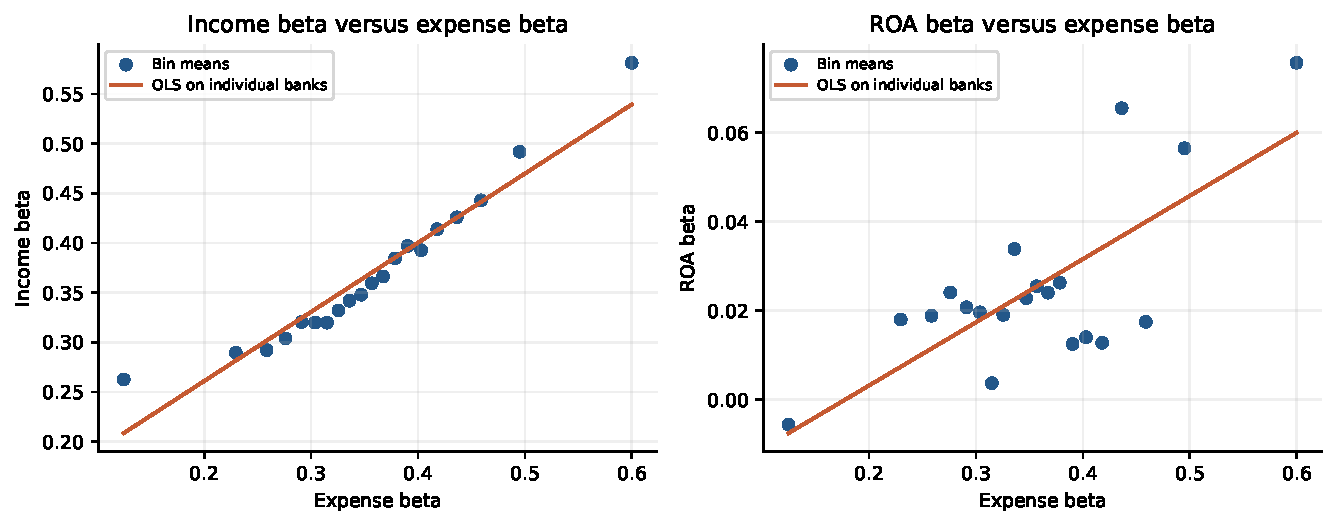
\includegraphics[width=0.92\textwidth]{figures/beta_relationships.pdf}
\caption{Each point is the mean within an expense-beta quantile bin (20 bins). Lines are OLS fits to individual banks, displayed over the bin-mean range. Binning improves readability without removing beta outliers.}\label{fig:betas}
\end{figure}

\subsection*{C. Listed companies, share prices and returns}
I match \texttt{idrssd}, then \texttt{bhc\_id} when no direct match exists, to the link table's RSSD identifier, requiring its dates to cover the accounting quarter-end. Direct matches take priority; competing company links would be excluded (none remain). This links \LinkedBanks{} banks to \LinkedCompanies{} companies across the accounting sample. After requiring valid stock observations, complete accounts and publication timing, \MarketBanks{} banks contribute to \MarketCompanies{} listed companies and \MarketObservations{} company--months, January 2000--December 2017. The supplied stock file starts in 2000.

For banks mapping to one company, I sum total assets, equity, quarterly average assets and quarterly net income, then form ROA and capital ratios from those sums. I exclude \IncompleteGroups{} company--quarters with an invalid component among matched banks. Company size is log total assets; ROA and equity/assets are winsorized within quarter at 0.5\% and 99.5\%. These aggregates cover matched commercial subsidiaries, not consolidated holding-company accounts; missing subsidiaries, nonbank activities and intra-group positions limit coverage.

Actual filing dates are unavailable. I assume accounts become public 120 days after quarter-end and use only reports whose assumed availability strictly precedes the return month. Reports older than one year are excluded. Links must remain valid through that month; records are not carried beyond a reported parent change. This conservative timing rule reduces look-ahead risk but cannot verify late filings or subsequent data revisions.

I retain US ordinary common shares listed on NYSE, AMEX or Nasdaq, using security classifications valid at the return month's start.\footnote{Field mapping and ordinary-share classification follow the \href{https://wrds-www.wharton.upenn.edu/pages/wrds-research/macros/crsp-ciztosiz-macro/}{WRDS CRSP CIZ-to-SIZ documentation}.} Repeated security--month rows are removed only after confirming identical return and capitalization fields (\StockDuplicates{} duplicates). Missing or invalid returns and nonpositive or stale prior-month market capitalizations are excluded; valid returns, including $-100\%$, are not trimmed. Multiple share classes are combined using prior-month capitalization weights.

Figure~\ref{fig:prices} chains monthly ex-dividend returns, first within companies and then across the available accounting-linked companies, with the same prior-month capitalization weights. December 1999 equals 100. This produces a comparable price index rather than averaging dollar share prices; it excludes cash dividends and changes composition as firms enter or exit. The series falls sharply during the financial crisis and recovers to \MarketLastIndex{} by December 2017.

\begin{figure}[H]
\centering
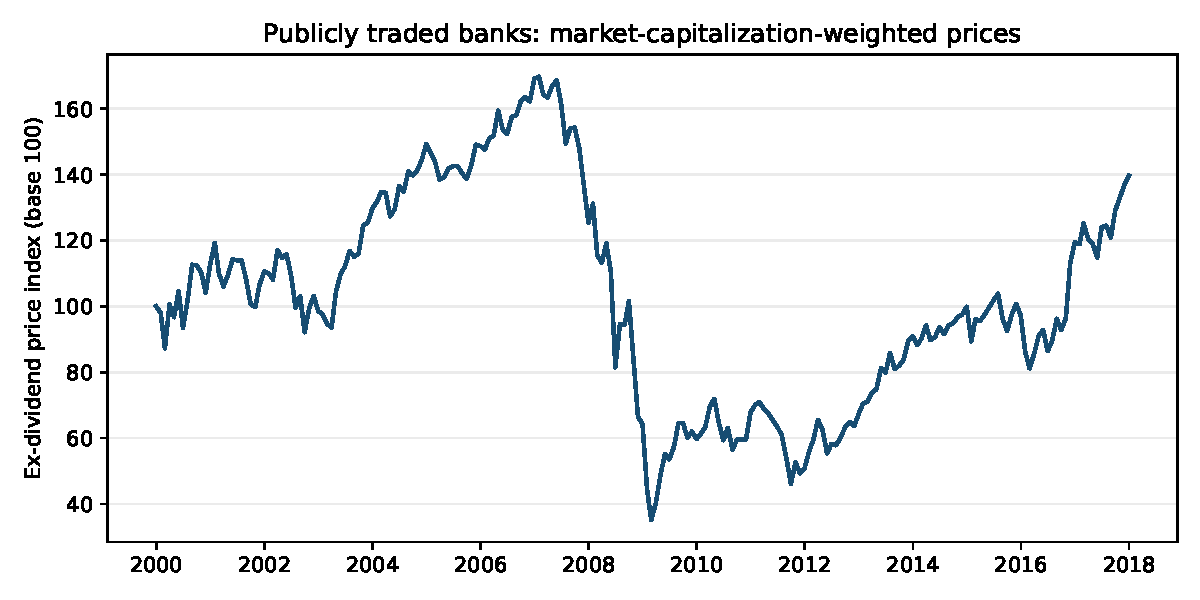
\includegraphics[width=0.80\textwidth]{figures/bank_stock_price_index.pdf}
\caption{Ex-dividend price index for companies with usable prior accounting data. December 1999 = 100.}\label{fig:prices}
\end{figure}

For monthly total stock return $r_{cm}$ in percentage points, I estimate
\[
 r_{cm}=\alpha_c+\lambda_m+\theta_1\log(Assets_{c,q(m)})
       +\theta_2ROA_{c,q(m)}+\theta_3Capital_{c,q(m)}+e_{cm},
\]
where $q(m)$ denotes the latest eligible prior report. Company effects absorb persistent differences; month effects absorb common market movements. Standard errors are clustered by company and month to allow serial and contemporaneous dependence. The coefficients describe within-company associations conditional on common monthly shocks; a separate intercept is absorbed by the fixed effects.

\begin{table}[H]
\centering
\caption{Company characteristics and subsequent monthly stock returns}\label{tab:market}
\begin{tabular}{lr}
\toprule
 & Monthly return (pp) \\
\midrule
Log assets & -0.628 \\
 & (-3.74) \\
Annualized ROA (pp) & 0.034 \\
 & (0.31) \\
Equity/assets (pp) & -0.043 \\
 & (-2.42) \\
Company and month effects & Yes \\
Company-months & 64,230 \\
Companies & 691 \\
Adjusted $R^2$ (including effects) & 0.175 \\
\bottomrule
\end{tabular}

\begin{minipage}{0.85\textwidth}\footnotesize
OLS with company and month fixed effects; $t$-statistics use two-way clustered standard errors. ROA and equity/assets are in percentage points. Assets are measured in nominal USD thousands before taking logs. Adjusted $R^2$ includes the fixed effects.
\end{minipage}
\end{table}

A one-log-unit increase in assets is associated with a \StockSize{} pp change in monthly returns; a 1 pp increase in equity/assets is associated with a \StockCapital{} pp change. Lower capital can coincide with greater leverage and risk compensation, but the estimates do not establish that mechanism. The ROA coefficient is \StockRoa{} pp per 1 pp of ROA and is imprecise. Accounting performance need not predict returns when prices already incorporate it. These are conditional associations, not a trading strategy or causal estimates; reporting delays, incomplete company coverage and changes in risk remain relevant.

\paragraph{Time spent (reported).}
Part 1: 20 minutes. Part 2: 1.5 hours. Part 3: 1.5 hours.

\end{document}
